% Files using this must be two subfolders
% deep. Adjust the number of ../ for the
% depth of the file.
% Imports
\usepackage{fancyhdr}
\usepackage{geometry}
\usepackage{icomma}
\usepackage{amsmath}
\usepackage{multicol}
\usepackage{mathptmx}
\usepackage{anyfontsize}
\usepackage{t1enc}
\usepackage{tabto}
\usepackage{listings}
\usepackage{filecontents}
\usepackage{subcaption}
\usepackage{tikz}
\usepackage[parfill]{parskip}
\usepackage{graphicx}
\usepackage[]{mdframed}
\usepackage{amsmath}
\usepackage[makeroom]{cancel}
\usepackage{pgfplots}
\usepackage{pgfplotstable}
\usepackage{xfrac}
\usepackage{amssymb}
\usepackage{mathtools}
\pgfplotsset{compat=1.18}
\usetikzlibrary{patterns}
\usepgfplotslibrary{polar}
\usepgfplotslibrary{fillbetween}

\geometry{margin=2.5cm}

\newcommand{\name}{Kaleb Burris}
\newcommand{\classname}{MATH F253, Elizabeth S. Allman, University of Alaska Fairbanks}
\newcommand{\assignment}{FILL IN ASSIGNMENT NAME}

\pagestyle{fancy}

\fancyhead[L]{
    \name 
    \newline
    \classname
    \newline
    \assignment
}

\newcommand{\horizontal}{\noindent\rule{\hsize}{0.4pt}}

\setlength{\headheight}{42pt}
\setlength{\headsep}{0.25in}
\setlength{\columnsep}{0.35cm}
\setlength{\columnseprule}{1pt}

\usepackage[T1]{fontenc}
\usepackage{lmodern}

\usepackage{enumitem}
\usepackage{graphicx}
\graphicspath{ {./lab02images/} }

% Put class number, class name, and professor 
% name.
% Use only in case of emergency, this
% should be covered by the preamble.
% \renewcommand\classname{}

% Put the assignment name with \S if 
% necessary for the section and the question 
% numbers.
\renewcommand\assignment{Lab 2: Acceleration and Force, 2/7/2023, Partners: Maite Valentin-Lugo, Seth Waln}

\begin{document}

    % Templates
    \iffalse
    % Use these for equations.
    \begin{equation*}
        \begin{gathered}
            Equations go here.
        \end{gathered}
    \end{equation*}

    % Use this if a line of math is too long.
    \resizebox{\hsize}{!}{$Long equation goes here$}

    % Use these for multiple columns.
    \begin{multicol*}{# of columns}
        % Remove the * if you want the columns to be balanced.
    \end{multicol*}

    % Use this to add a horizontal line.
    \horizontal

    \fi

    % Begin homework here.
    %%%%%%%%%%%%%%%%%%%%%%

    \section*{Part 1: Speeding Up}

    \paragraph*{1.}

    \begin{mdframed}
        \begin{equation}
            \vec{a} = \frac{\mathrm{d}\vec{v}}{\mathrm{d}t}
        \end{equation}

        Acceleration is the derivative of velocity; it describes the rate of change of the velocity.

        \begin{equation}
            \sum\vec{F} = m\vec{a}
        \end{equation}

        Forces are a sum or integral of the mass and acceleration applied to something.
    \end{mdframed}

    \paragraph*{2.}

    \begin{mdframed}
        \centering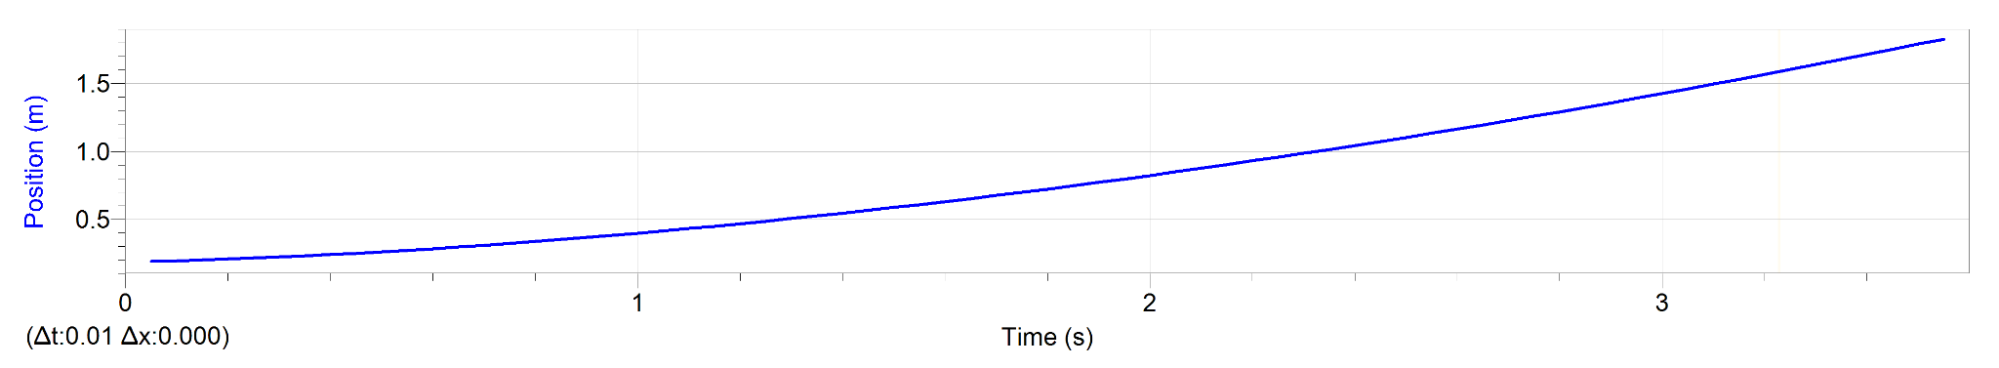
\includegraphics[width=\textwidth]{image17}
        \centering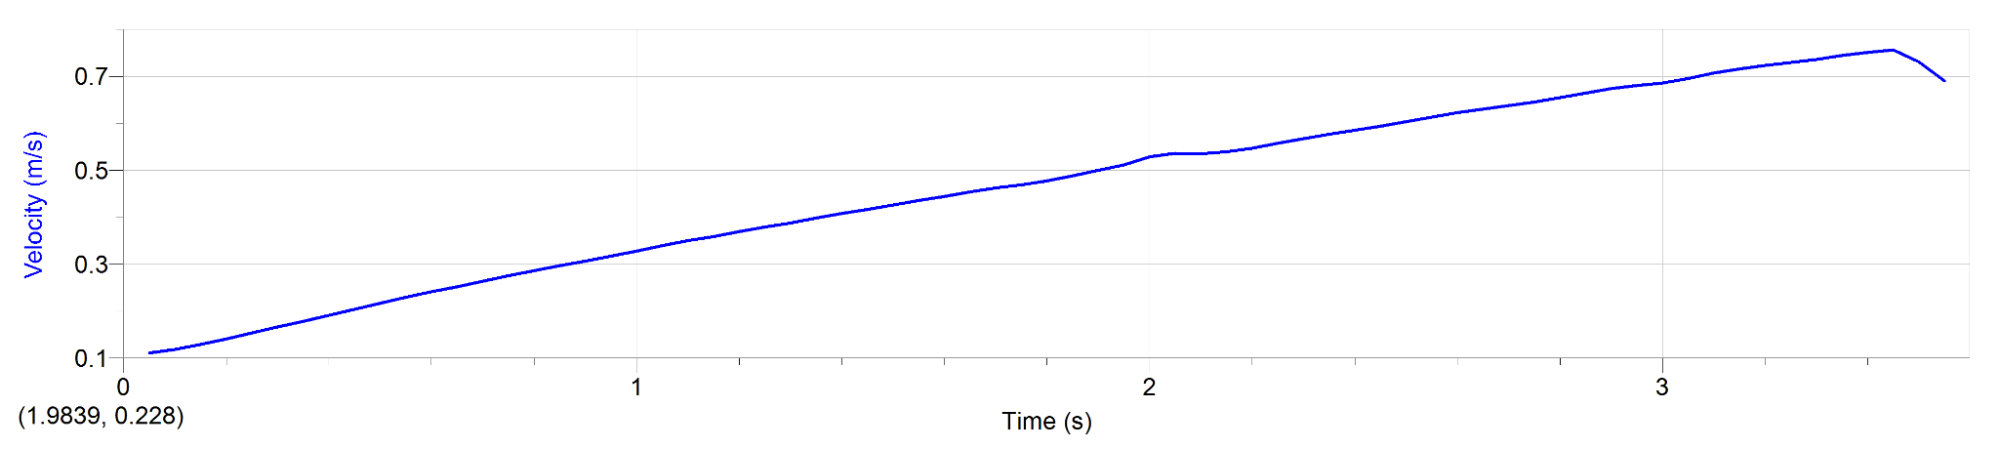
\includegraphics[width=\textwidth]{image10}
        \centering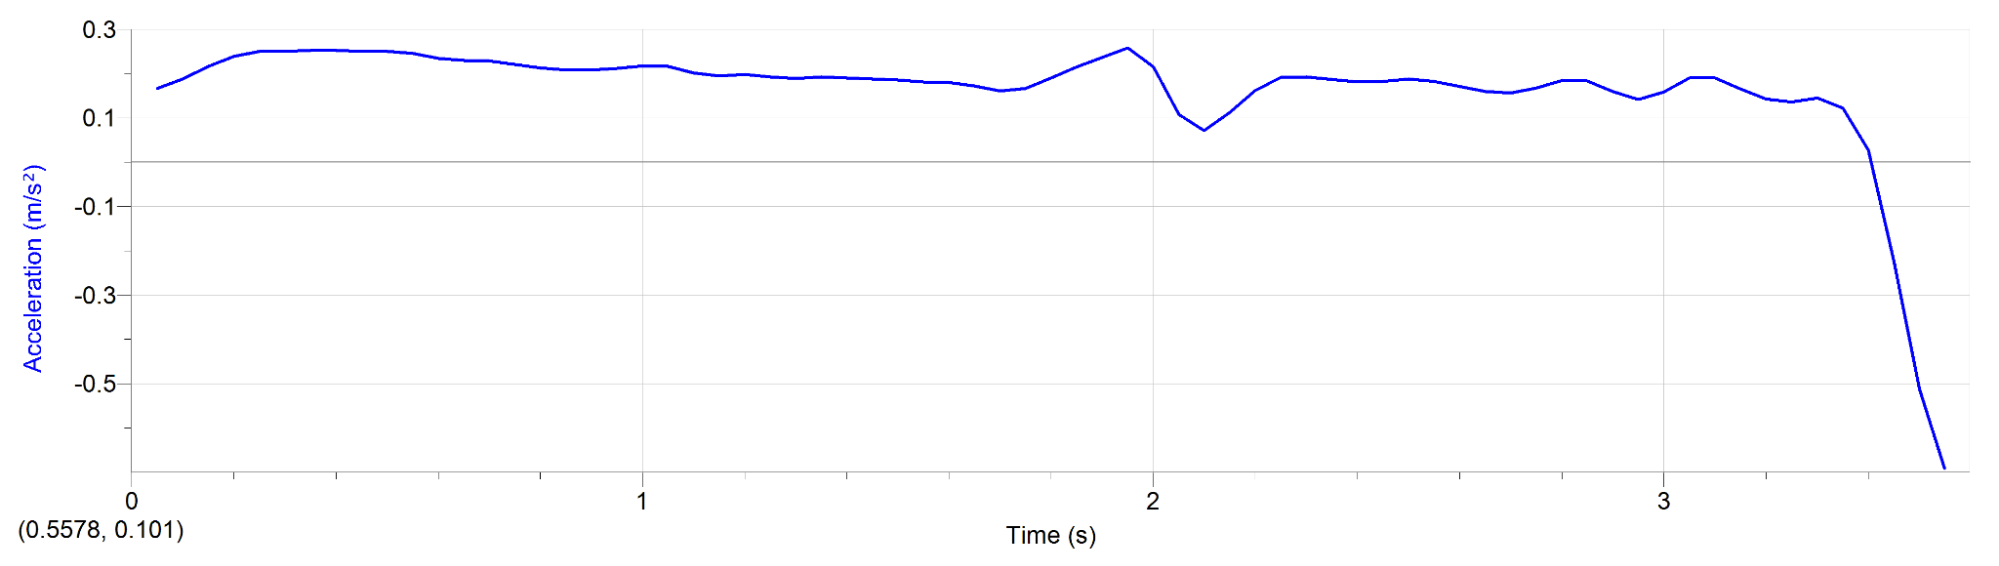
\includegraphics[width=\textwidth]{image7}
    \end{mdframed}

    \paragraph*{3.}

    \begin{mdframed}
        Statistics for: Latest | Acceleration

        min: 0.07098 at 2.100 max: 0.2578 at 1.950

        mean: 0.1908 median: 0.1899

        std. dev: 0.03808 samples: 67

        $\Delta y$: 0.187       
    \end{mdframed}

    \paragraph*{4.}

    \begin{mdframed}
        If the initial mass is doubled, the acceleration will be doubled, making the velocity increase at twice the rate and resulting in the cart traveling the same distance in $\sim\sfrac{1}{4}$ the time.
    \end{mdframed}

    \paragraph*{5.}

    \begin{mdframed}
        \centering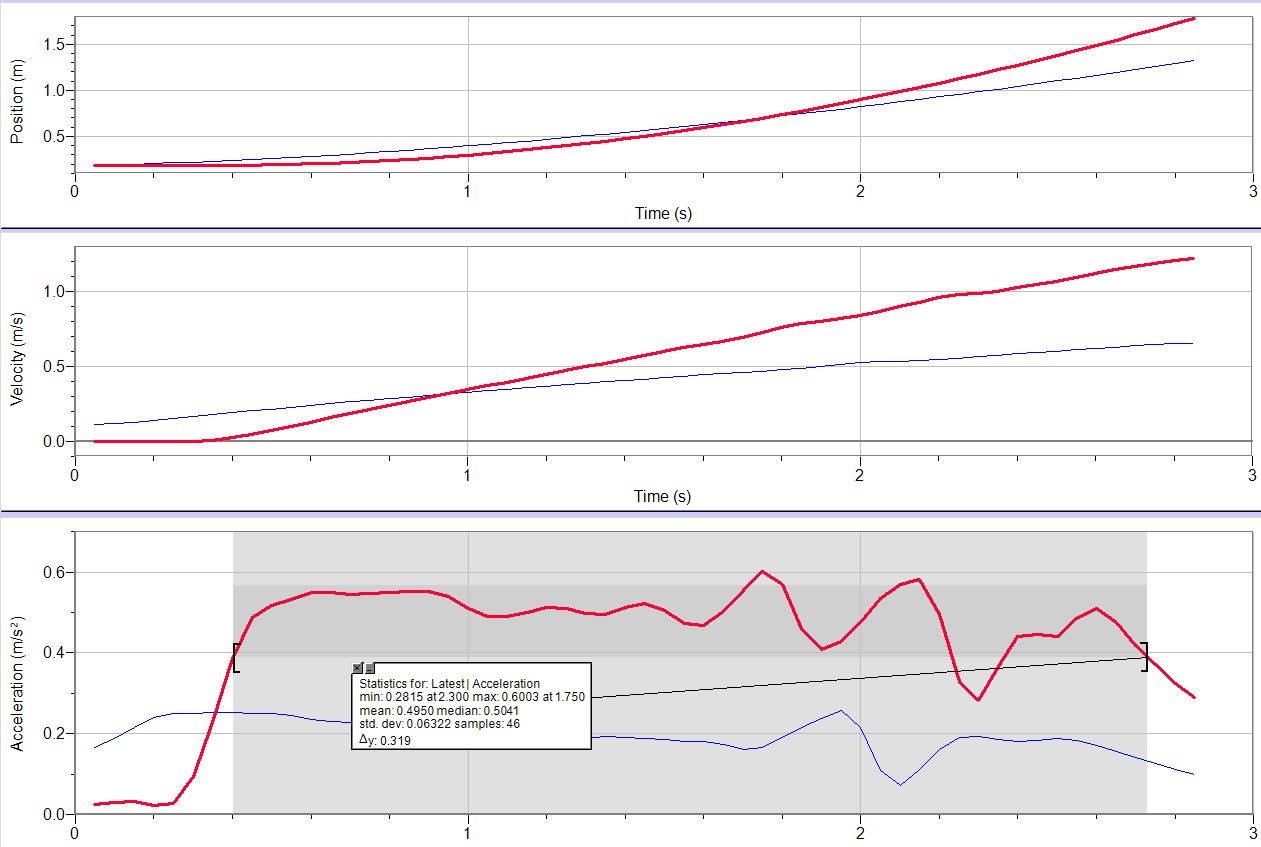
\includegraphics[width=\textwidth]{image12}
    \end{mdframed}

    \pagebreak

    \section*{Part 2: Slowing Down}

    \paragraph*{6.}

    \begin{mdframed}
        The acceleration would be negative because the cart will decelerate to a stop, with the vector of the deceleration being pointed toward the sensor.
    \end{mdframed}

    \paragraph*{7.}

    \begin{mdframed}
        {\centering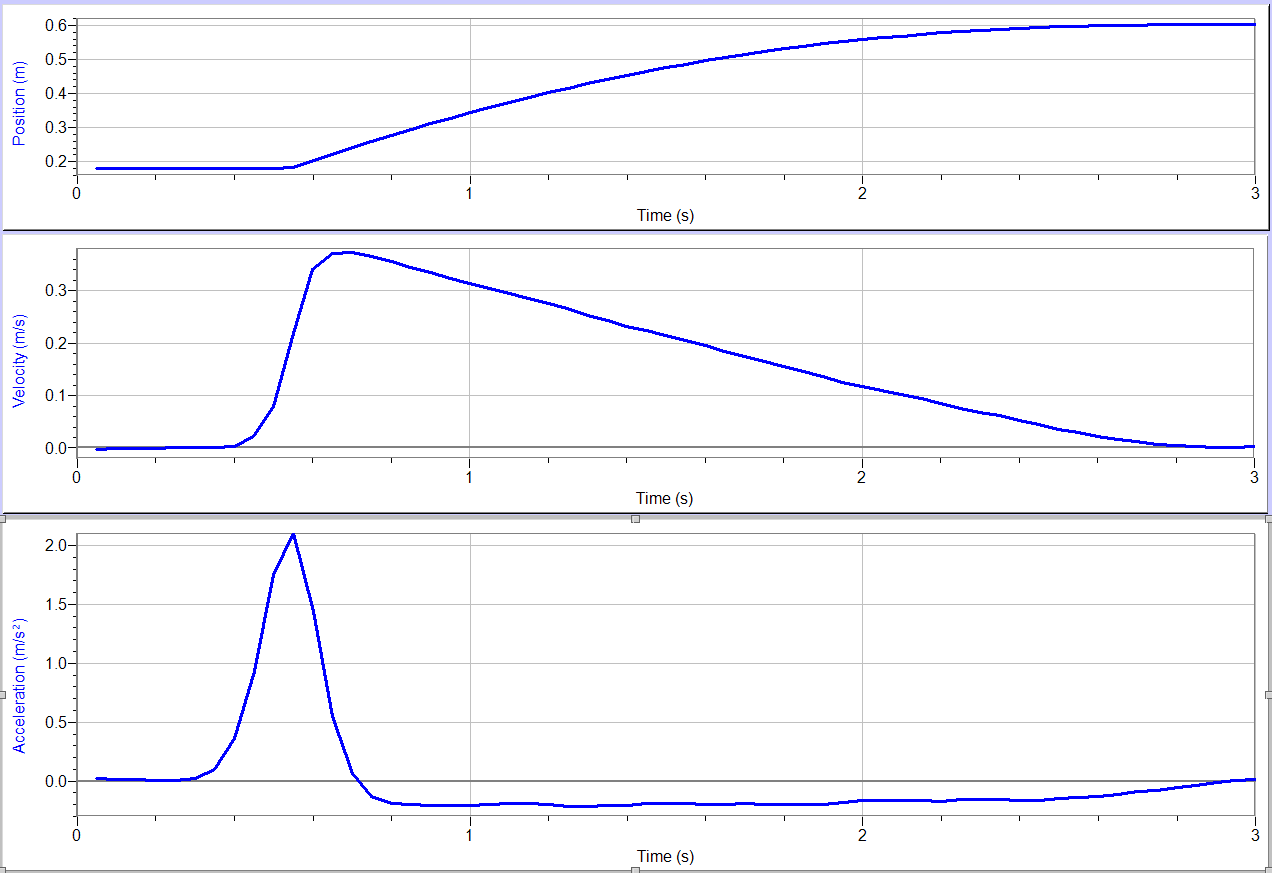
\includegraphics[width=\textwidth]{image13}}

        Statistics for: Latest | Acceleration

        min: -0.2118 at 1.250 max: 0.01807 at 3.000

        mean: -0.1586 median: -0.1858

        std. dev: 0.06011 samples: 45

        $\Delta y$: 0.230       
    \end{mdframed}

    \pagebreak

    \section*{Part 3: Force}

    \paragraph*{8.,9.,10.}

    \begin{mdframed}
        {\centering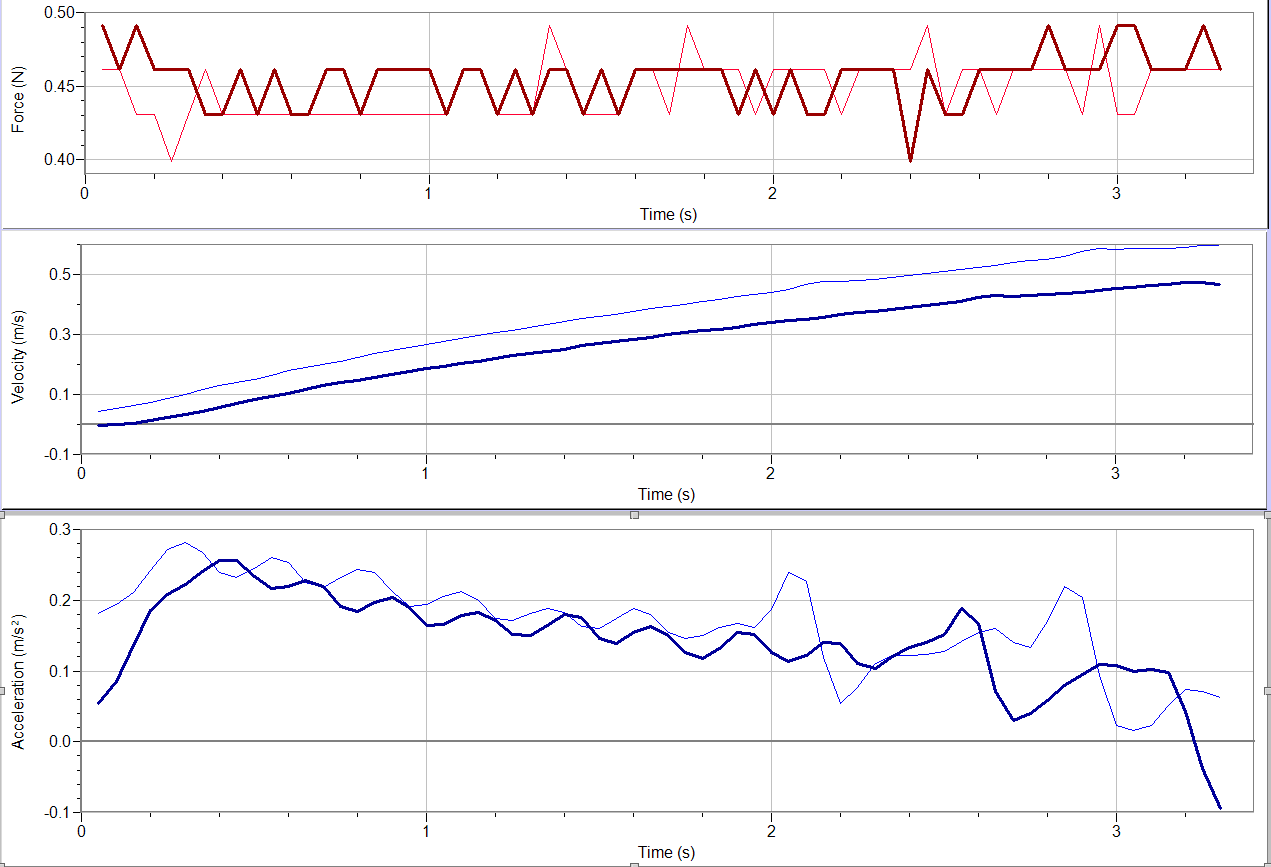
\includegraphics[width=\textwidth]{image16}}

        The lighter lines are the ``no-friction'' experiment.

        \subparagraph*{8.}
        For force, there seems to be little to no difference - although this may have been because of the inaccuracy of the recording device.

        \subparagraph*{9.}
        For velocity, there seems to be a slight advantage for the no-friction experiment which grows a small amount as it approaches the end.
        
        \subparagraph*{10.}
        For acceleration, there seems to be a very slight advantage for the no-friction experiment.
    \end{mdframed}

    \pagebreak

    \paragraph*{11.}

    \begin{mdframed}
        {\centering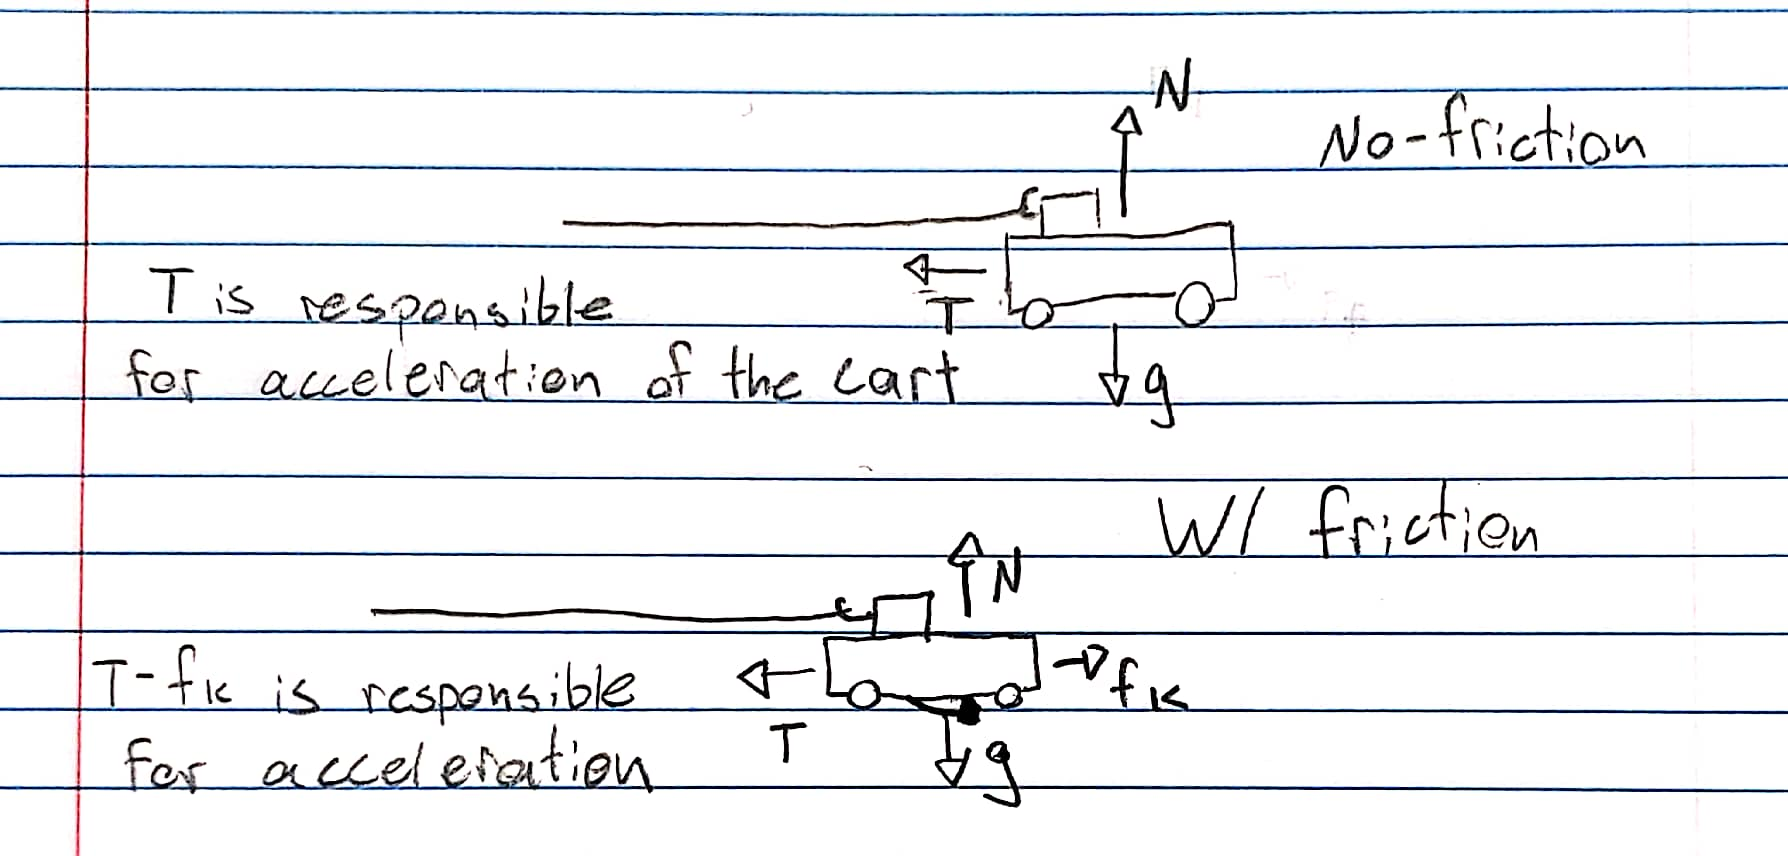
\includegraphics[width=\textwidth]{image5}}
    \end{mdframed}

    \paragraph*{12.}

    \begin{mdframed}
        The acceleration will be doubled if the weight is doubled.
    \end{mdframed}

    \paragraph*{13.}

    \begin{mdframed}
        {\centering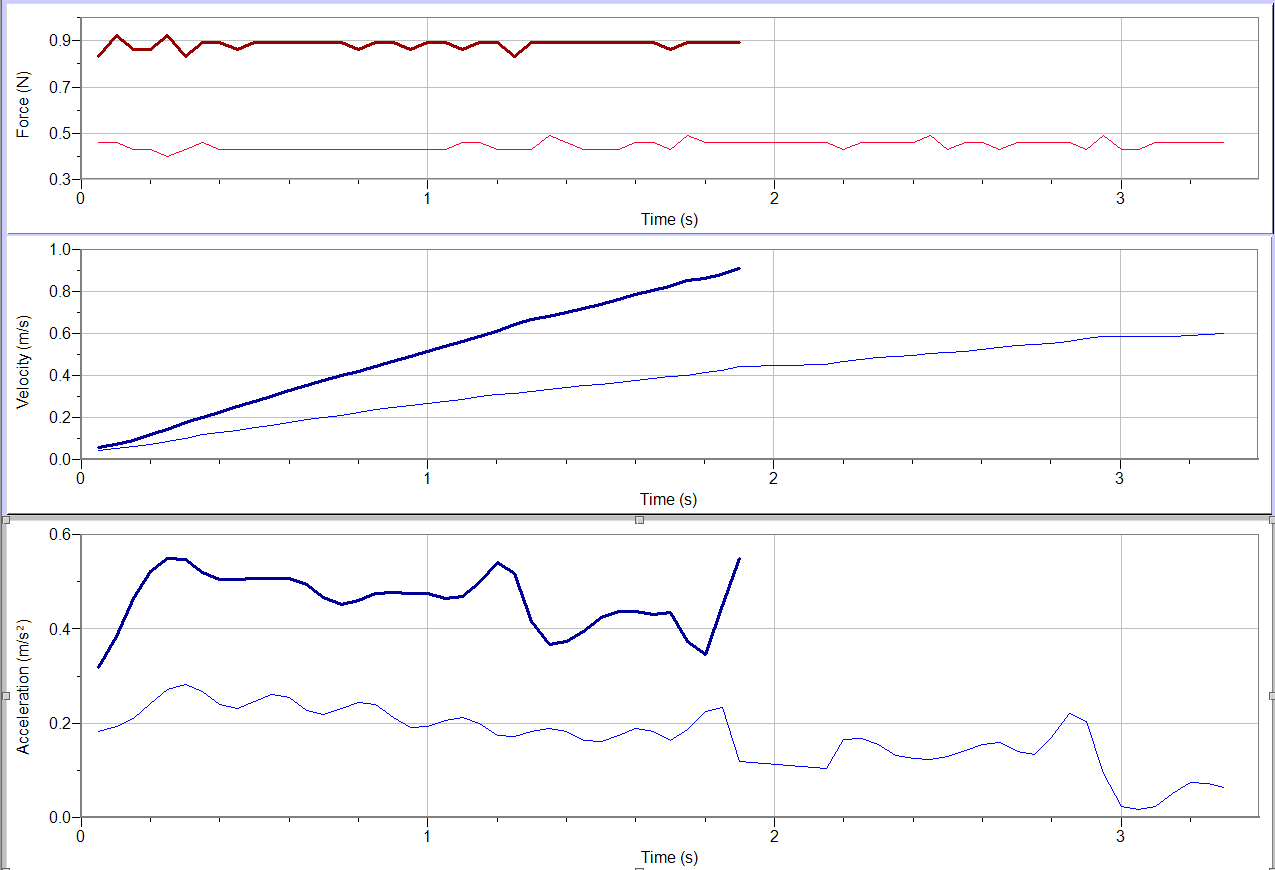
\includegraphics[width=\textwidth]{image6}}
    \end{mdframed}

    \section*{4: Velocity and acceleration of a cart on an inclined plane}

    \paragraph*{14., 15.}

    \begin{mdframed}
        {\centering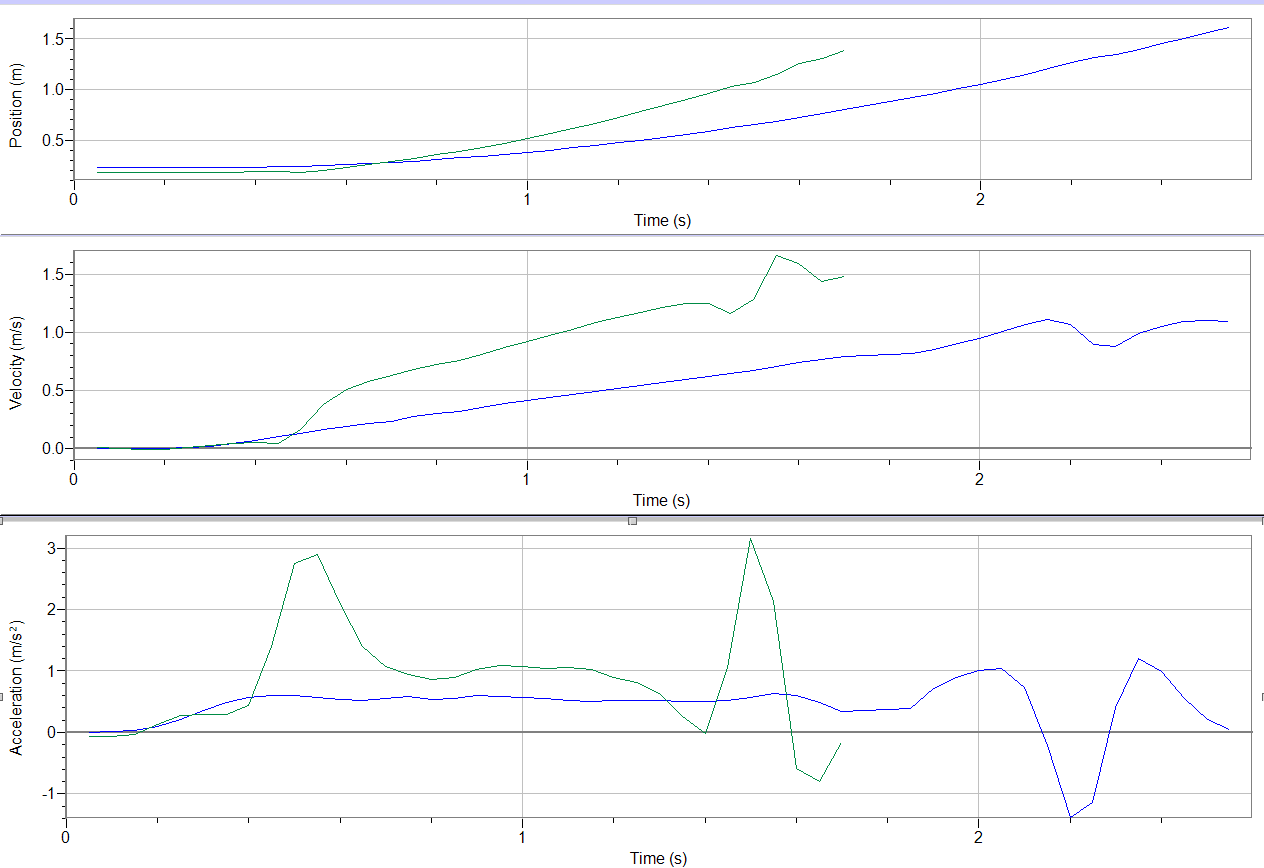
\includegraphics[width=\textwidth]{image14}}

        At a steeper slope, the acceleration was higher which resulted in the velocity and position having steeper slopes, this resulted in reaching the end of the ramp in $\sim\sfrac{2}{3}$ the time of the shallower slope.
    \end{mdframed}

    \pagebreak

    \paragraph*{16., 17.}
    
        
    \begin{mdframed}
            \begin{multicols}{2}
            \centering\begin{tikzpicture}[scale=0.8]
                \begin{axis}[
                    axis lines=middle,
                    axis line style={->},
                    x label style={at={(axis description cs:0.5,-0.1)},anchor=north},
                    y label style={at={(axis description cs:-0.1,.5)},rotate=90,anchor=south},
                    xlabel={time $s$},
                    ylabel={velocity $\vec{v}$},
                    ymin=-2,ymax=2,
                    xmin=0,xmax=5
                ]
                    \draw[red] (0,-2) -- (5,2);
                    \node[anchor=south] at (2.5,1.2){Top of ramp};
                    \draw[->] (2.5, 1.2) -- (2.5, 0.25);
                    \node[circle, inner sep=0, minimum size=5pt, fill=black] at (2.5,0){};
                \end{axis}
            \end{tikzpicture}

            \columnbreak

            \centering\begin{tikzpicture}[scale=0.8]
                \begin{axis}[
                    axis lines=middle,
                    axis line style={->},
                    x label style={at={(axis description cs:0.5,-0.1)},anchor=north},
                    y label style={at={(axis description cs:-0.1,.5)},rotate=90,anchor=south},
                    xlabel={time $s$},
                    ylabel={acceleration $\vec{a}$},
                    ymin=-4,ymax=3,
                    xmin=0,xmax=5
                ]
                    \draw[red] (0,0) .. controls(1,-2) .. (2.5,0);
                    \draw[red] (2.5,0) .. controls (3.75, 2) .. (5, 2);
                    \node[anchor=south] at (2.5,2){Top of ramp};
                    \draw[->] (2.5, 2) -- (2.5, 0.25);
                    \node[circle, inner sep=0, minimum size=5pt, fill=black] at (2.5,0){};
                \end{axis}
            \end{tikzpicture}
        \end{multicols}
    \end{mdframed}

    \paragraph*{18., 19.}
    
    \begin{mdframed}
        {\centering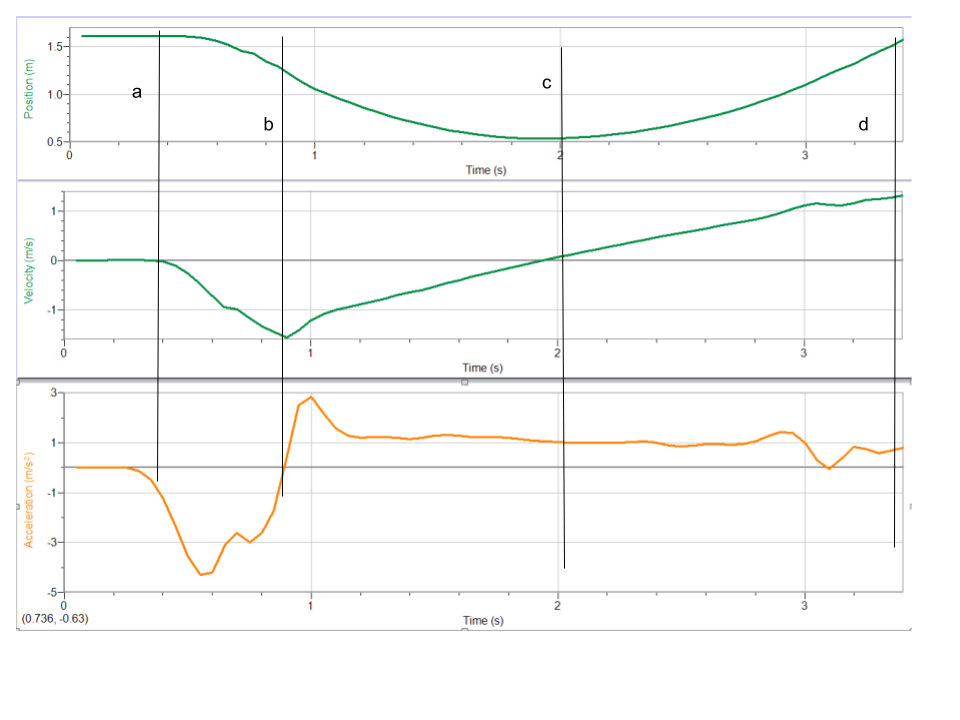
\includegraphics[width=\textwidth]{image21}}
    \end{mdframed}

    \pagebreak

    \paragraph*{20.}
    
    \begin{mdframed}
        {\centering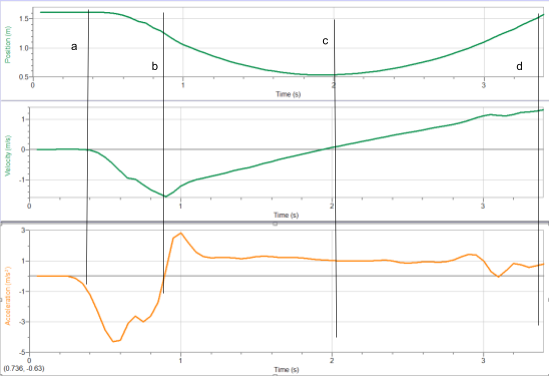
\includegraphics[width=\textwidth]{image9}}
    \end{mdframed}

    \section*{Conclusion Questions}

    \paragraph*{21.}

    \begin{mdframed}
        Motion away is represented as a positive value. Speeding up is signified by a positive/negative slope to the velocity graph.
    \end{mdframed}

    \paragraph*{22.}

    \begin{mdframed}
        The magnitude of the acceleration is the absolute value of the slope of the plot.
    \end{mdframed}

    \paragraph*{23.}

    \begin{mdframed}
        The magnitude of the acceleration is represented as the absolute value of the acceleration vs time graph.
    \end{mdframed}

    \paragraph*{24.}

    \begin{mdframed}
        The sign of the velocity is positive and the sign of the acceleration is negative because the cart is moving in the positive direction but accelerating in the negative direction.
    \end{mdframed}

    \paragraph*{25.}

    \begin{mdframed}
        The force is relatively even but does have a slight peak towards the end of the ramp, probably due to the stopping of the cart.
    \end{mdframed}

    \paragraph*{26.}

    \begin{mdframed}
        The force does not change with or without the friction pad, but the acceleration does. This is not a violation because there is an extra force being applied to the cart that isn't being detected by the probe - friction - that forces either the mass of the object or the acceleration to change according to $\sum F = m\vec{a}$ as the net force changes on the cart.
    \end{mdframed}

    \paragraph*{27.}

    \begin{mdframed}
        The velocity shoots to a negative value and then returns on a linear path to a positive one; the acceleration shoots sharply down and then returns up to a positive constant. My graphs were pretty close but failed to capture the start-up of the velocity graph and the extra peaks/troughs of the acceleration graph.
    \end{mdframed}

    \paragraph*{28.}

    \begin{mdframed}
        \begin{enumerate}[label=\Alph*.]
            \item The average velocity on the way up is positive.
            \item The acceleration on the way up is negative.
            \item At the top, the velocity is zero.
            \item At the top the acceleration is negative.
            \item The velocity on the way down is negative.
            \item The acceleration on the way down is negative.
            \item When the ball's velocity and acceleration have opposite signs the ball is \underline{going up} and when the velocity and acceleration have the same sign the ball is \underline{falling down}.
        \end{enumerate}
    \end{mdframed}

    \paragraph*{29.}

    \begin{mdframed}
        When the friction pad is down, it applies a force that will constantly affect the acceleration, especially while the cart is rolling down the ramp.

        \centering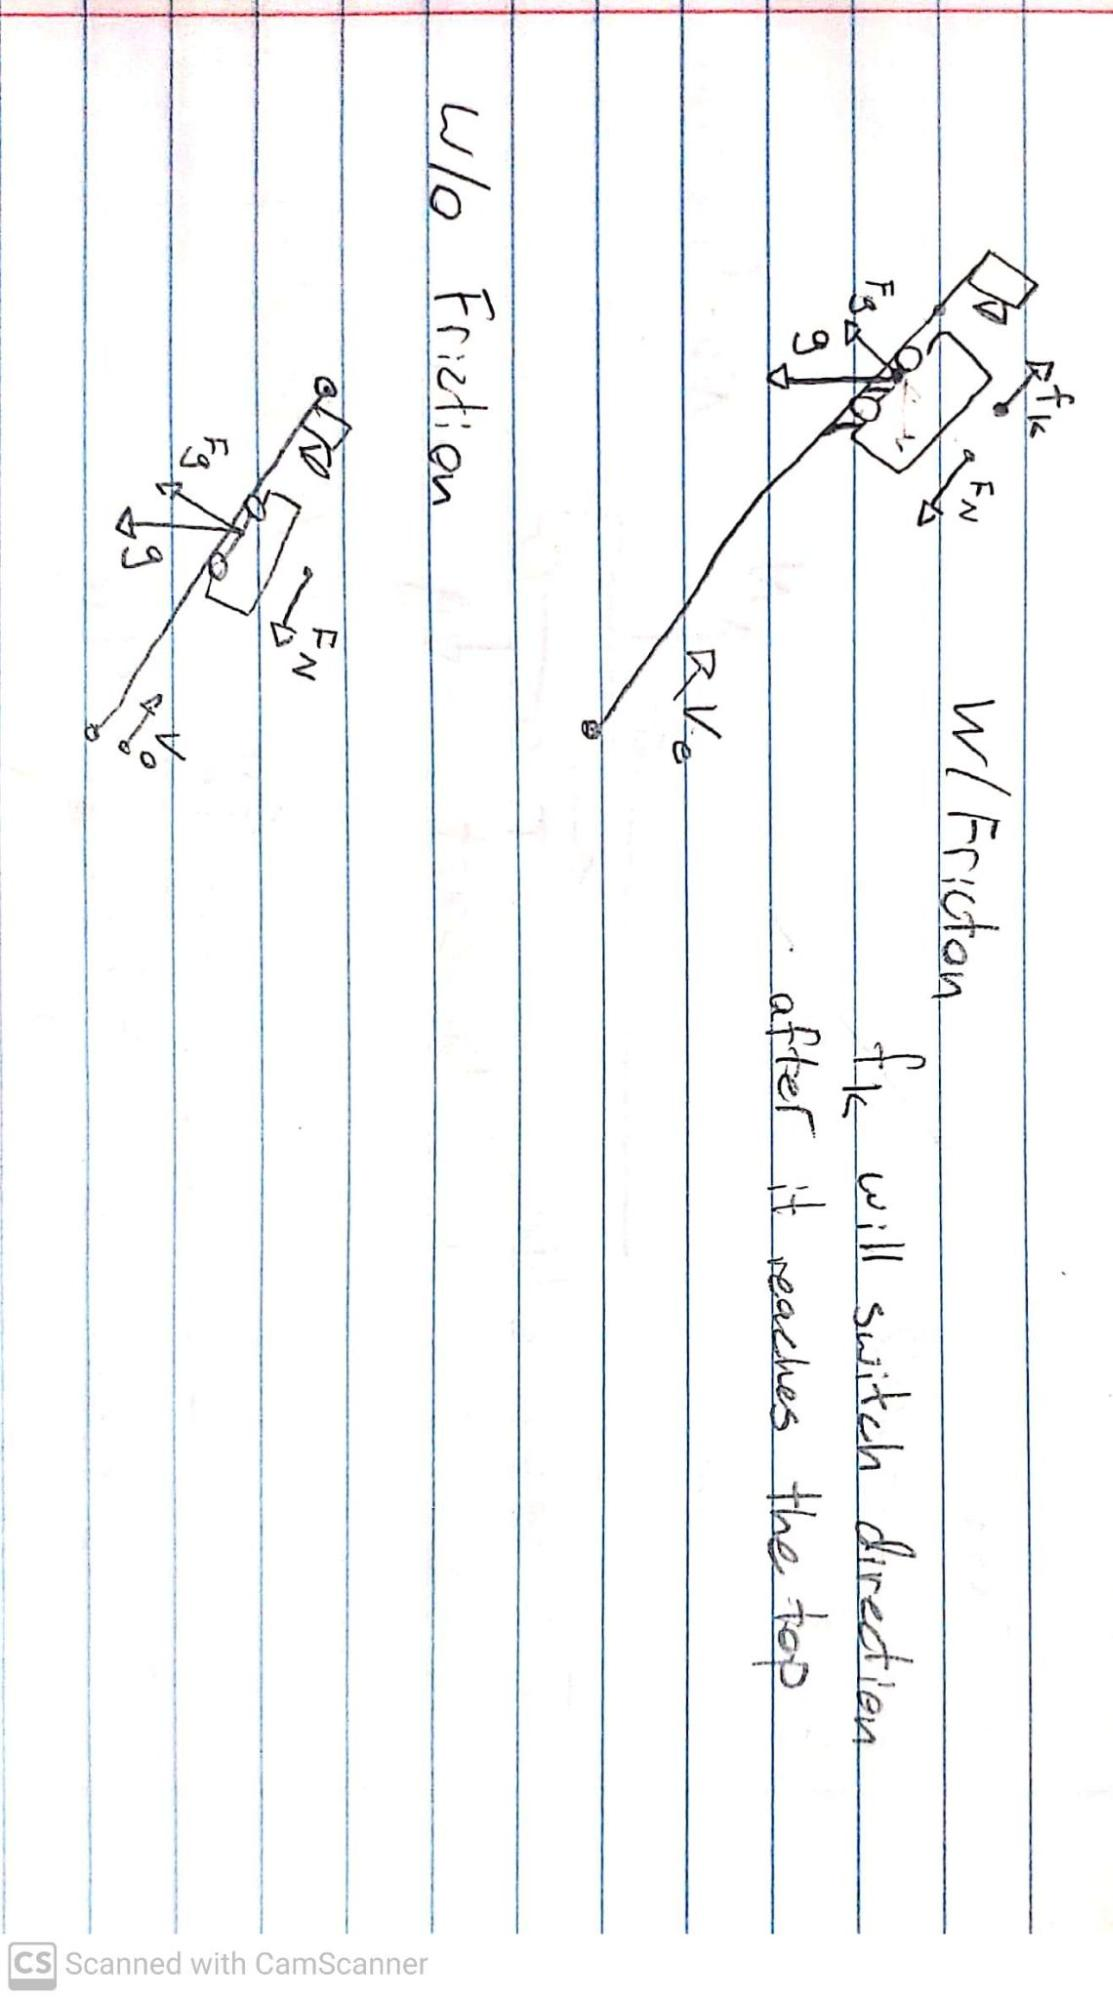
\includegraphics[angle=90,origin=c,width=0.6\textwidth]{image4}
    \end{mdframed}

\end{document}